\chapter{Восстановление филогенетических деревьев из брейкпоинт графа}

\section{Получение информации из брейкпоинт графа}
Описанные в предыдущей главе методы вычисления редакционного расстояния между геномами можно рассмотреть в ином ключе.
Редакционное расстояние в модели методов основанных на расстояниях \q{стягивает} геномы друг к другу, заставляя их находиться ближе в дереве, то есть,
принимается, что геномы с меньшим редакционным расстоянием находятся в одном поддереве с большей вероятностью.
Иными словами, расстояние дает нам филогенетическую информацию о ветвях в филогенетическом дереве.

В~\cite{xu2010exploring} автор рассматривает несколько оценок редакционного расстояния, включая описанные выше
и вводит концепцию филогенетического паттерна позволяющую применять их к восстановлению деревьев из брейкпоинт графа.
\begin{define}{Филогенетический паттерн} \\
  Филогенетический паттерн $P(\bb{G}, T)$, где $\bb{G}$ - множество геномов,
  а $T$ - топология филогенетического дерева на них - функция, которая для данных входных геномов
  сопоставляет каждой из возможных топологий филогенетического дерева эвристическую оценку так,
  чтобы она была максимальной только на одной топологии.
\end{define}
Главное свойство данной концепции в том, что имея на руках листовые геномы филогенетического дерева, можно получить всегда только одно возможное дерево.
Тогда если найти филогенетический паттерн, который будет давать максимальное значение на тех же топологиях,
что и другая оценка $s$ (например, $d_{BP}$), то он будет давать ту же филогенетическую информацию, что и $s$.
Получается, что имея на руках паттерн, то становится возможным получать оптимальное дерево с точки зрения использованной оценки.
Более того, возможно определить множество паттернов, каждый из которых, в общем случае, может давать максимальное значение на разных топологиях,
для этого для каждого из паттернов необходимо определить тот вес, который он вносит в оценку, для каждого паттерна это будет рассмотрено отдельно.
Wei Xu показал, что филогенетические паттерны удобно строить на основе подграфов брейкпоинт графа,
так как зачастую информации (значения оценки) получаемой на основе малых подграфов достаточно для того,
чтобы отличить разные топологии филогенетического дерева и восстановить корректное.
В дальнейшем филогенетический паттерн и подграф на котором он вычисляется будут использоваться взаимозаменяемо.
Рассмотрим предложенный Wei Xu паттерн \q{контрастирующая смежность}.
\begin{figure}[H]
  \centering
  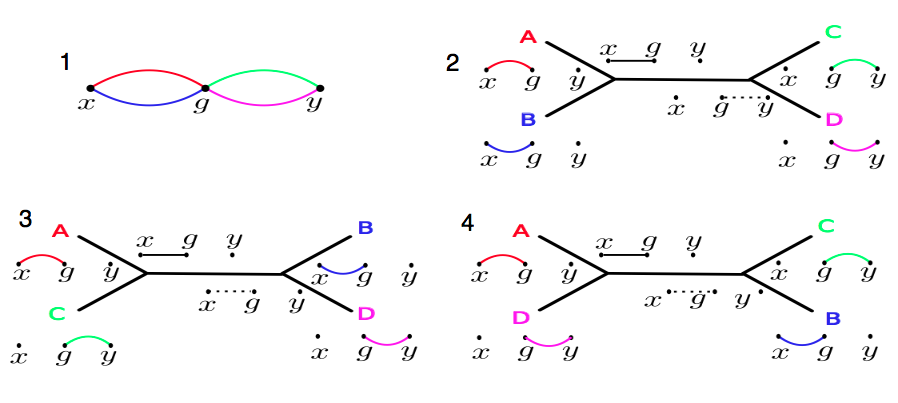
\includegraphics[max width=\linewidth]{fig/2/contrasting_adjacency.png}
  \caption{Контрастирующая смежность~\cite{xu2010exploring}}
  \label{fig:contrasting_adjacency}
\end{figure}
Этот паттерн представляет собой подграф брейкпоинт графа из трех вершин, где одна пара соединена двумя ребрами цветов $A$ и $B$, а другая - $C$ и $D$.
Обозначим, что для 4 геномов $A, B, C, D$, $AB|CD$ обозначает, что геномы $A$ и $B$ находятся в одном поддереве, а $C$ и $D$ - в другом.
Тогда для топологии $AB|CD$ можно посчитать расстояние $d (d_{DCJ}, d_{BP})$ как $d(A, B) + d(C, D) + d(I_1, I_2)$,
где $d(\_, \_)$ - функция расстояния между двумя геномами, $I_1, I_2$ - предки в дереве на парах геномов $AB$ и $CD$ соответственно.
Из рисунка~\ref{fig:contrasting_adjacency} можно увидеть, что на топологии $AB|CD$ оценки $d_{BP}$ и $d_{DCJ}$, полученные как указано выше, достигают минимального значения.
Вышеописанный паттерн был обобщен для многих геномов в~\cite{Alekseyev2009} с помощью концепции \textit{простого пути}.
\begin{define}{Простой путь} \\
  Простой путь - путь в брейкпоинт графе, состоящий из вершин мультистепени 2 и ребер двух альтернирующих
  (меняющих друг друга по ходу движения по ребрам) мультицветов $Q$ и $Q'$, таких что $Q \cap Q' = \varnothing \land Q \cup Q' = \bb{Q}$,
  где $\bb{Q}$ - множество всех цветов.
\end{define}

Заметим что, каждый филогенетический паттерн по сути дает лишь часть филогенетической информации, закодированной в брейкпоинт графе.
Основываясь на предыдущем замечании, можно понять, что информация извлеченная из брейкпоинт графа будет тем точнее,
чем больше непересекающихся (не использующих одни и те же основания для различия топологий) паттернов будет найдено.
Так, становится необходимым искать филогенетические паттерны в графах, для чего необходимо определить, какие паттерны искать.

Определение паттернов вручную - тяжелый и медленный процесс, потому в данной работе предложен метод их автоматического поиска.
Филогенетический паттерн - это подграф в брейкпоинт графе, раскрашенный в несколько цветов.
Важно заметить два факта:
\begin{enumerate}
  \item Каждый цвет в данном случае необязательно соответствует одному геному, но может соответствовать целой их группе.
  \item Если взять ребра одного цвета из подграфа образующего филогенетический паттерн, то они не будут вершинно пересекаться и образуют паросочетание.
\end{enumerate}

Первый факт важен для получения информации с помощью филогенетических паттернов из брейкпоинт графов для многих геномов,
а второй позволяет перейти к автоматическому поиску филогенетических паттернов.
Ниже представлен алгоритм такого поиска.
\begin{enumerate}
  \item Выбрать с повторениями 4 паросочетания, как конфигурации геномов.
  \item Для каждой из 3 топологий перебрать паросочетания для внутренних вершин (они тоже являются паросочетаниями).
  \item Выбрать те кортежи из 4 геномов, на которых оценка достигает экстремума.
\end{enumerate}

Важно заметить, что алгоритм выше выполняет перебор, без проверки на уникальность найденных графов, потому необходимо удалить \q{похожие} из них.
Для этого можно определить понятие \textit{изоморфизма паттернов}.
\begin{define}{Изоморфизм паттернов} \\
  Паттерны $A$ и $B$ изоморфны тогда и только тогда, когда существует пара биективных отображений $(f, h)$,
  $f$ - между вершинами паттерна $A$ вершинами паттерна $B$, $h$ - между ребрами паттерна $A$ и ребрами паттерна $B$,
  такая что любые две вершины $u$ и $v$ в $A$ связаны мультимножеством раскрашенных ребер $E$ тогда и только тогда, когда вершины
  $f(u)$ и $f(v)$ связаны $h(E)$.
\end{define}
\vspace{-2em}
\begin{figure}[H]
  \centering
  \minipage{0.25\textwidth}
  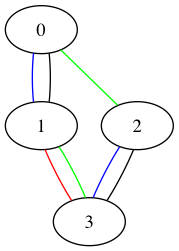
\includegraphics[max width=\linewidth]{fig/2/patterns/similar1.png}
  \endminipage
  \minipage{0.25\textwidth}
    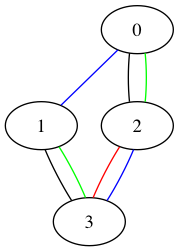
\includegraphics[max width=\linewidth]{fig/2/patterns/similar2.png}
  \endminipage
  \caption{Изоморфные паттерны}
  \label{fig:isomorphic_patterns}
\end{figure}

Таким образом, могут быть найдены все паттерны на любом количестве вершин.
В данной работе были найдены паттерны, показанные на рисунках~\ref{fig:cylinder_pattern} и~\ref{fig:bag_pattern}.
\begin{figure}[H]
  \centering
  \minipage{0.25\textwidth}
  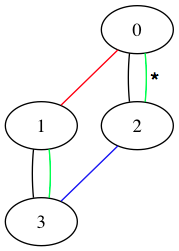
\includegraphics[max width=\linewidth]{fig/2/patterns/cylinder.png}
    \caption{Паттерн \q{цилиндр}}
    \label{fig:cylinder_pattern}
  \endminipage \hspace{1em}
  \minipage{0.25\textwidth}
  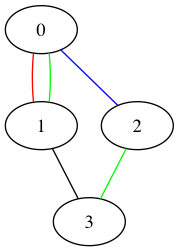
\includegraphics[max width=\linewidth]{fig/2/patterns/bag.png}
    \caption{Паттерн \q{мешок}}
    \label{fig:bag_pattern}
  \endminipage
\end{figure}

\section{Сборка деревьев из разделений}
Смысл использования филогенетических паттернов для восстановления деревьев заключается в том,
чтобы извлечь информацию о устройстве филогенетического дерева из брейкпоинт графа в удобном для восстановления виде.
Так каждая копия филогенетического паттерна найденная в брейкпоинт графе дает информацию о том,
что одна часть геномов находятся ближе друг к другу, а другие - дальше друг от друга в филогенетическом дереве.
Например, если в графе встречается паттерн \q{простой путь} на двух альтернирующих цветах $Q_1$ и $Q_2$, то он \q{свидетельствует},
что геномы из множества $Q_1$ находятся в одном поддереве, а геномы из множества $Q_2$ - в другом.
Таким образом, механизм филогенетических паттернов позволяет получить из брейкпоинт графа информацию о ветвях филогенетического дерева.
Сформулируем задачу восстановления филогенетического дерева из полученной информации.
Для этого введем понятие \textit{разделения} как единицы информации об устройстве филогенетического дерева.
\begin{define}{Разделение} \\
  Пусть $\bb{Q}$ - множество всех листовых геномов.
  Разделение - пара множеств вида $Q_1|Q_2$, таких, что $Q_1 \subset \bb{Q}$ и $Q_2 \subset \bb{Q}$ и при этом
  $Q_1 \cap Q_2 = \varnothing$ и $Q_1 \cup Q_2 = \bb{Q}$.
\end{define}
Введем обозначения что для разделения вида $D = Q_1|Q_2$, $left(D) = Q_1$, $right(D) = Q_2$.
Также заметим, что для дальнейшего использования разделения $Q_1|Q_2$ и $Q_2|Q_1$,
где $Q_1$, $Q_2$ - подмножества множества всех геномов $\bb{Q}$, идентичны.

Представим каждое вхождение паттерна $P$ в брейкпоинт граф как разделение $Q_1|Q_2$,
если согласно вхождению паттерна $P$ геномы $Q_1$ должны находиться в одном поддереве результирующего филогенетического дерева,
а геномы $Q_2$ - в другом.
Таким образом, имея набор искомых паттернов и брейкпоинт граф, можно преобразовать последний в список вхождений паттернов в него,
после чего получить набор разделений $\bb{D}$.
В таком случае все разделения считаются одинаково ценными и неясно, как восстановить дерево из них, так как непонятно,
как выбирать из двух противоречащих друг другу разделений то, которое должно войти в результирующее дерево,
потому введем понятие \textit{статистики}.
\begin{define}{Статистика}\\
  Статистика - разделение с оценкой.
\end{define}
Под оценкой в данном случае подразумевается то, насколько весомо \q{свидетельство} о данном разделении:
например, простой путь длины $l$ дает свидетельство в $\lfloor\frac{l}{2}\rfloor$ единиц.
Далее, сгруппируем все статистики с одинаковыми разделениями и сложим их оценки.
Тогда мы получим множество статистик $\bb{S} = \{(D, V)\}$, где каждое разделение $D$ встречается не больше одного раза.
Обозначим, что для статистики $S = (D, V)$, $D = div(S)$ и $V = value(S)$.
Сформулируем теперь задачу, решение которой даст нам лучшее восстановленное дерево из возможных на основе выделенной филогенетической информации.
\begin{task}{Восстановление из статистик} \\
  Восстановить филогенетическое дерево с наилучшей оценкой имея на входе набор статистик,
  полученных из брейкпоинт графа.
\end{task}

В данной работе будет описано два алгоритма сборки деревьев из полученных статистик:
наивный алгоритм и реализация динамическим программированием.
Для описания алгоритмов введем отношение \textit{непересечения} между двумя разделениями.
\begin{define}{Непересекающиеся разделения} \\
  Два разделения $Q_1|Q_2$ и $R_1|R_2$ \textit{не пересекаются},
  если $Q_1 \cap R_1 = \varnothing \lor Q_1 \cap R_2 = \varnothing $.
  Отношение непересечения симметрично.
\end{define}

\subsection{Наивный алгоритм}
Суть данного алгоритма в том, чтобы перебрать все деревья, о которых \q{свидетельствует} брейкпоинт граф и выбрать из них лучшее.
Стоит также заметить, что в данном алгоритме перебираются не все \emph{возможные} деревья, но только те, о которых \q{свидетельствует} брейкпоинт граф,
что, в зависимости от способа извлечения филогенетической информации из брейкпоинт графа, может значительно уменьшить перебор.
Введем понятие \textit{класса непересекающихся разделений}, которое описывает возможное дерево в виде разделений.
\begin{define}{Класс непересекающихся разделений} \\
  Класс непересекающихся разделений $D_i$ - подмножество множества всех разделений $\bb{D}$,
  в котором любые два разделения не пересекаются между собой.
\end{define}

\noindent Таким же образом определим понятие \textit{класса непересекающихся статистик}.
\begin{define}{Класс непересекающихся статистик}\\
  Класс непересекающихся статистик $S_i$ - подмножество множества всех статистик $\bb{S}$,
  такое что $\forall S \in S_i: div(S) \in D_i$,
  где $D_i$ -  класс непересекающихся разделений.
\end{define}

\noindent Для класса непересекающихся статистик $S_i$ определим его оценку \\
$V_i = \sum\nolimits_{S \in S_i} value(S)$.

\begin{define}{Максимальный класс непересекающихся разделений} \\
  Будем называть класс непересекающихся разделений $D_i$ \textit{максимальным},
  если в него невозможно добавить новое разделение из множества разделений $\bb{D}$,
  так чтобы он сохранил свойство непересечения.
\end{define}

\begin{define}{Максимальный класс непересекающихся статистик} \\
  Максимальный класс непересекающихся статистик - класс непересекающихся статистик $S_i$,
  такое что $\forall S \in S_i: div(S) \in D_i$,
  где $D_i$ - максимальный класс непересекающихся разделений.
\end{define}


Заметим, что из исходного множества разделений, в общем случае, можно получить несколько максимальных классов непересекающихся разделений.
\begin{example}
  Рассмотрим случай, что $\bb{D} = \{ AB|CD, AC|BD, A|BCD \}$, где $A, B, C, D$ - геномы.
  В данном случае можно получить максимальные классы непересекающихся разделений
  $D_0 = \{ AB|CD, A|BCD \}$ и $D_1 = \{ AC|BD, A|BCD \}$.
\end{example}
Из этого примера также видно, что разделение может входить в различные классы, что соответствует тому случаю, когда
одна ветвь присутствует в разных деревьях.


Заметим также, что из класса непересекающихся разделений можно собрать дерево единственным образом.
Здесь и далее под деревьями подразумеваются некорневые бинарные деревья с помеченными листьями,
для их представления используется формат Newick~\cite{newick} с фиктивным корнем,
поддеревья с неизвестной внутренней топологией обозначаются как $\{A, B, C\}$,
где $A, B, C$ - геномы, топология дерева для которых неизвестна.
\begin{example}
  Пусть есть класс непересекающихся разделений $D_0 = \{AB|CDEF,$ $ABC|DEF\}$, где $A, B, C, D, E, F$ - геномы.
  Используя трактовку разделений, что разделение вида $Q_1|Q_2$ обозначает то, что геномы из множества $Q_1$ лежат в левом поддереве,
  а геномы из множества $Q_2$ - в правом, можно получить два дерева, удовлетворяющих требованиям разделений из $D_0$:
  \begin{itemize}
    \item $((\{AB\}, C), \{DEF\});$
    \item $(\{AB\}, (C, \{DEF\}));$
  \end{itemize}
  Если рассматривать эти деревья в постановке описанной выше, то становится ясно, что они одинаковы.
  \begin{figure}[H]
    \centering
    \minipage{0.35\textwidth}
    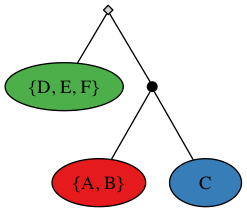
\includegraphics[max width=\linewidth]{fig/2/similar_tree1.png}
      \caption{$((\{AB\}, C), \{DEF\});$}
    \endminipage
    \minipage{0.35\textwidth}
      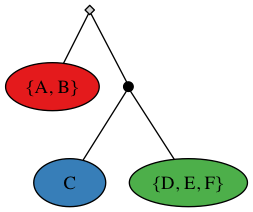
\includegraphics[max width=\linewidth]{fig/2/similar_tree2.png}
      \caption{$(\{AB\}, (C, \{DEF\}));$}
    \endminipage
  \end{figure}
  Закрашенный кружок обозначает предка, ромб обозначает фиктивный корень.
\end{example}


На основе вышеизложенного сформулируем наивный алгоритм:
\begin{enumerate}
  \item Выделить среди статистик множество максимальных классов непересекающихся $\bb{C}$
  \item Отсортировать множество $\bb{C}$ по убыванию оценки
  \item Выбрать лучший по оценке класс
  \item Выделить разделения из статистик выбранного класса и собрать из них дерево
\end{enumerate}

\subsection{Реализация динамическим программированием}

Проблемой предыдущего алгоритма являлось то, что он выполнял перебор всех деревьев, о которых \q{свидетельствует} брейкпоинт граф,
в случае многих геномов таких деревьев может быть много, что приведет к тому, что работа алгоритма может занять большое время.
Предположим, что для любой статистики $S$ с разделением вида $Q_1|Q_2$ из некоторого набора $\bb{S}$ известны поддеревья с наилучшей оценкой,
построенные на множествах геномов $Q_1$ и $Q_2$, тогда чтобы найти дерево с максимальной оценкой нужно перебрать все статистики из $\bb{S}$ и найти ту,
оценка которой в сумме с оценками поддеревьев даст наибольшее значение.
Данную логику можно применить также для того, чтобы построить оптимальные деревья для вышеупомянутых пар множеств $Q_1$ и $Q_2$,
составляющих разделения статистик.
Таким образом, приходим к задаче динамического программирования для решения которой сформулируем следующий алгоритм:
\begin{enumerate}
  \item Обозначим, что для любого множества $F$ размера $f$, $size(F) = f$.
    Пусть даны множества $\bb{G}$ геномов и $\bb{S}$ имеющихся статистик.
    Введем структуру множеств $\{ SCLevel_i | i = 1..N \}$, где $N = size(\bb{G})$,
    a $\forall i, SCLevel_i$ - множество четверок вида $(C, V, V, ())$, таких что $size(C) = i$,
    $\exists S \in \bb{S}: (C = left(S) \lor C = right(S)) \land value(S) = V$.
    Компоненты четверки обозначают соответственно: множество геномов, на котором построено дерево;
    оценку этого множества; суммарную оценку построенного дерева; пару множеств геномов, лежащих в левом и правом поддеревьях.
  \item Начиная с $i = 2$,
    $\forall c = (C, V, CS, SS) \in SCLevel_i$,
    $(C1, \_, CS1, \_) \in SCLevel_j$,
    $(C2, \_, CS2, \_) \in SCLevel_k$ обозначим, что $c = (C, V, V + CS1 + CS2, (C1, C2))$,
    если $V + CS1 + CS2$ - максимальное значение при условии  $j = 1..i-1$, $k = i - j$ и $C1 \cup C2 = C \land C1 \cap C2 = \varnothing$
  \item Пусть единственный элемент $SCLevel_N$ имеет вид $(\_, \_, \_, (C1, C2))$ тогда результирующее дерево можно построить сверху
    вниз для множеств $C1$ и $C2$, после чего объединить результаты корнем.
    Для множеств $C1$ и $C2$ можно выполнить сборку тем же образом, базой для индукции послужит случай,
    когда $C1$ и $C2$ - множества с одним элементом.
\end{enumerate}

\subsection{Примечания к практической реализации}

В первой главе были описаны недостатки существующих решений, которые не позволяли бы им работать с блоками, полученными из геномов со вставками
и удалениями, несобранными геномами или использовать для восстановления информацию об известных поддеревьях восстанавливаемого дерева.
Опишем, как предложенный подход борется с данными проблемами.

Рассмотрим, что происходит с брейкпоинт графом при работе с данными в которых происходили вставки или удаления блоков,
рассмотрим только случай циклических хромосом (в линейных различия будут случаться только в конечных блоках):
при удалении или вставке блока 2 вершины брейкпоинт графа теряют степень $N$ ($N$ - количество геномов), при вставке степень растет,
при удалении - падает.
Для того, чтобы ``не потерять'' структуры графа, зависящие от данных вершин в случае удаления блока выполняется добавление ``протезного'' ребра
необходимого цвета.
Далее статистики на графе считаются так же как и раньше, но к результирующим статистикам добавляется информация (в форме оценки) о том,
что было добавлено ребро такого цвета.

При работе с несобранными данными возникает проблема того, что при разбиении хромосомы собранного генома теряется одна смежность на каждые
два контига.
Данная потеря не наносит большого вреда, так как обычно при работе с несобранными геномами блоков много больше (зачастую на несколько порядков),
чем контигов, таким образом, потеря связностей из-за несобранности геномов мало влияет на процесс восстановления деревьев.

Чтобы поддержать работу с известными поддеревьями используется идея того, что любое разделение из известного поддерева должно присутствовать в результирующем.
Для того, чтобы обеспечить выполнение этого требования известное поддерево разбивается на разделения следующим образом:
\begin{enumerate}
  \item Пусть есть известное поддерево $(T, Q) = ((T_1, Q_1), (T_2, Q_2))$, где $T, T_1, T_2$ - бинарные деревья,
    а $Q, Q_1, Q_2$ - множества геномов в содержащиеся, $\bb{Q}$ - множество всех геномов,
    тогда для такого дерева набор разделений $Divisions(T)$ будет выглядеть как
    $\{Q|\bb{Q} \setminus  Q,$ $Q_1|\bb{Q} \setminus Q_1,$ $Q_2|\bb{Q} \setminus Q_2\} \cup Divisions(T_1) \cup Divisions(T_2)$,
    базой для данной индукции будет случай, когда $Q$ - множество из одного генома.
  \item Для каждого из полученных разделений назначаем оценку $\bb{V}=$ \\
    $\sum\nolimits_{S \in \bb{S}} value(S)$, где $\bb{S}$ - множество статистик, полученных из брейкпоинт графа.
\end{enumerate}
После таких операций каждое разделение из известного поддерева окажется в результате, так как при сборке любое пересекающееся с ним разделение
принесет меньше веса в оценку результирующего дерева и потому не будет взято.
